
\lstinputlisting[language=bash,basicstyle=\small]{python_codes/fieldstone_59/keywords}

\begin{center}
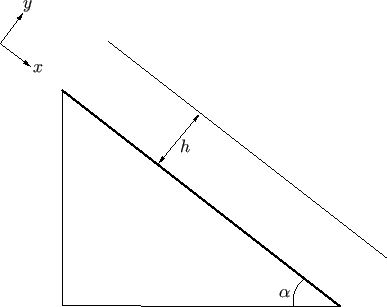
\includegraphics[width=5cm]{python_codes/fieldstone_59/images/setup}\\
{\captionfont REDO with tikz}
\end{center}

\paragraph{Linear viscous fluid}

We start from the Stokes equation for isoviscous fluids:
\[
\eta \Delta \vec{\upnu} - \vec\nabla p + \rho \vec{g} = \vec{\bm 0}
\]
Assuming that the fluid is incompressible and that the incline is infinite, 
then $\vec{\upnu}=(u(y),0)$.
The $x$-component of the equation then writes:
\[
\eta\left(\frac{\partial^2 u}{\partial x^2}+\frac{\partial^2 u}{\partial y^2} \right)
- \frac{\partial p}{\partial x} + \rho g_x =0
\]
\[
\Rightarrow \qquad 
\eta\frac{\partial^2 u}{\partial y^2} 
+ \rho g \sin\alpha =0
\]
since $\partial_x\rightarrow 0$.
This 2nd order ODE can be integrated twice. The two integration constants are 
determined by setting $u(y=0)=0$ (no slip) and the shear stress to be zero at the (free)
surface. The velocity profile is given by:
\[
u(y)=\frac{\rho g \sin \alpha}{2 \eta} (2h-y)y
\]
We can now compute the components of the strain rate tensor:
\[
\dot{\varepsilon}_{xx}=0
\qquad
\qquad
\dot{\varepsilon}_{yy}=0
\qquad
\qquad
\dot{\varepsilon}_{xy}
=\frac{1}{2} \left( \frac{\partial u}{\partial y} + \frac{\partial v}{\partial x} \right)
=\frac{1}{2} \frac{\partial u}{\partial y} 
= \frac{\rho g \sin \alpha}{2 \eta} (h-y)
\]

We now make the assumption that this problem is a very simplified ice sheet flow problem.
The angle $\alpha$ is typically small and for $\alpha\sim 0.5-1$\degree, then $\sin\alpha\sim 0.01$. 
We also have $\rho\sim1000$, $g\sim$10,  $h\sim2500$ and we postulate the 
ice viscosity to be $\eta\sim 10^m$,.
The velocity is maximum at the surface and is given by
\begin{equation}
u(y=h)=
\frac{\rho g \sin \alpha}{2 \eta}h^2 
\sim \frac{1000 \cdot 10 \cdot 0.01}{ 2\cdot 10^m}2500^2
\sim 3\cdot 10^{8-m}
\label{eq:ice1}
\end{equation}

\begin{center}
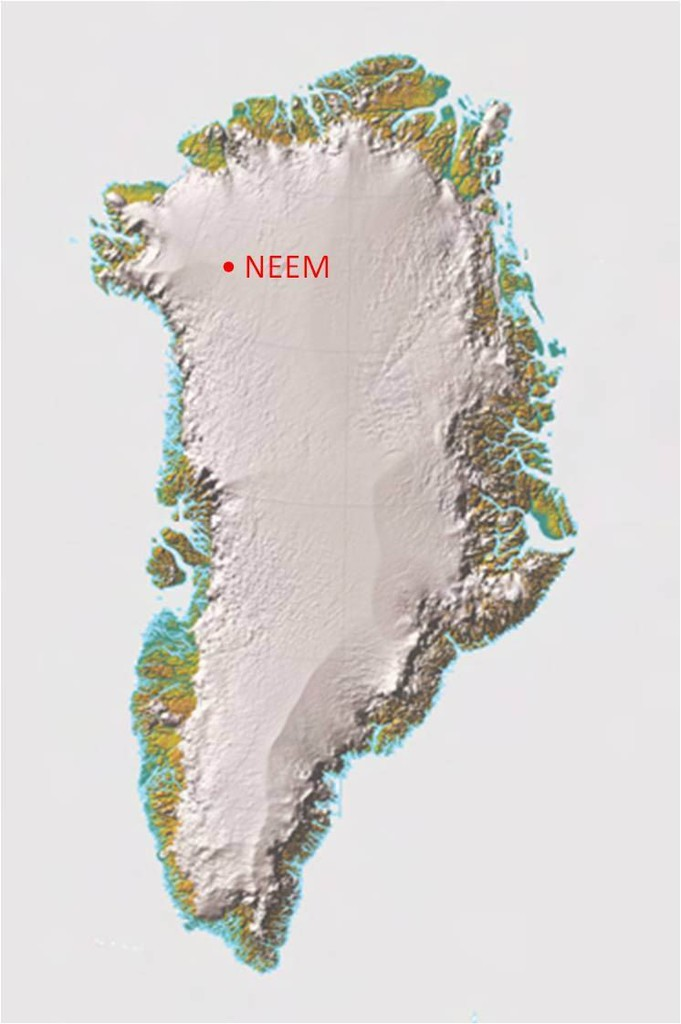
\includegraphics[height=9cm]{python_codes/fieldstone_59/images/neem}
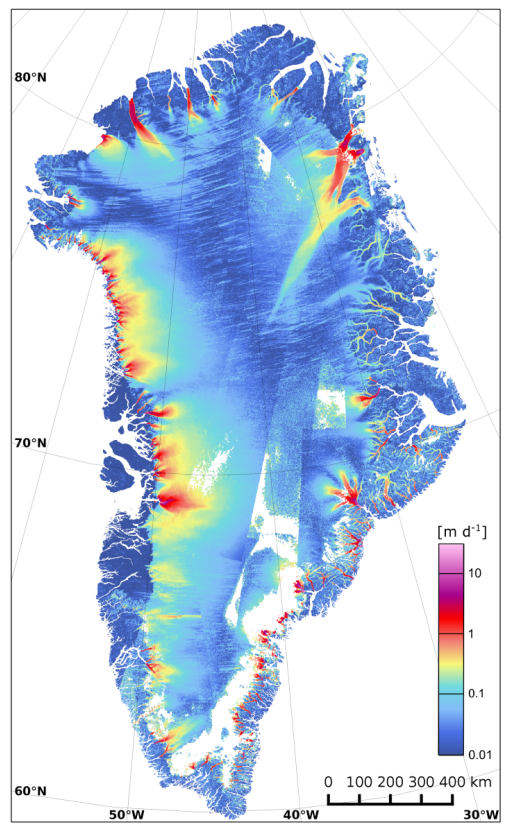
\includegraphics[height=9cm]{python_codes/fieldstone_59/images/narh15}\\
{\captionfont Ice velocity map (magnitude, in logarithmic scale) of the Greenland Ice Sheet
derived from SAR data of the Sentinel-1A satellite, acquired in Interferometric Wide Swath
Mode (IW) between January and March 2015. Taken from \cite{narh15}.}
\end{center}

As shown on the figures above the typical ice sheet velocity values around the NEEM ice core 
is $\sim 0.03m/day \simeq 3\cdot 10^{-7}$m/s. 
Then, in order for the top of the ice sheet to flow at this speed it requires $m=15$.

Having obtained the (effective linear) viscosity of the ice, i.e. $\eta\simeq 10^{15}$Pa.s,
we can compute the strain rate at the bottom and in the middle:
\[
\dot{\varepsilon}_{xy}(y=0) 
= \frac{\rho g \sin \alpha}{2 \eta} h
\sim \frac{1000\cdot 10 \cdot 0.01}{2 \cdot 10^{15}}2500
\sim 10^{-10}\text{s}^{-1}
\]
\[
\dot{\varepsilon}_{xy}(y=h/2) 
= \frac{\rho g \sin \alpha}{2 \eta} \frac{h}{2}
\sim \frac{1000\cdot 10 \cdot 0.01}{2 \cdot 10^{15}}\frac{2500}{2}
\sim 5\cdot 10^{-11}\text{s}^{-1}
\]
which are reasonable values as confirmed by the following figure (see yellow line):  
\begin{center}
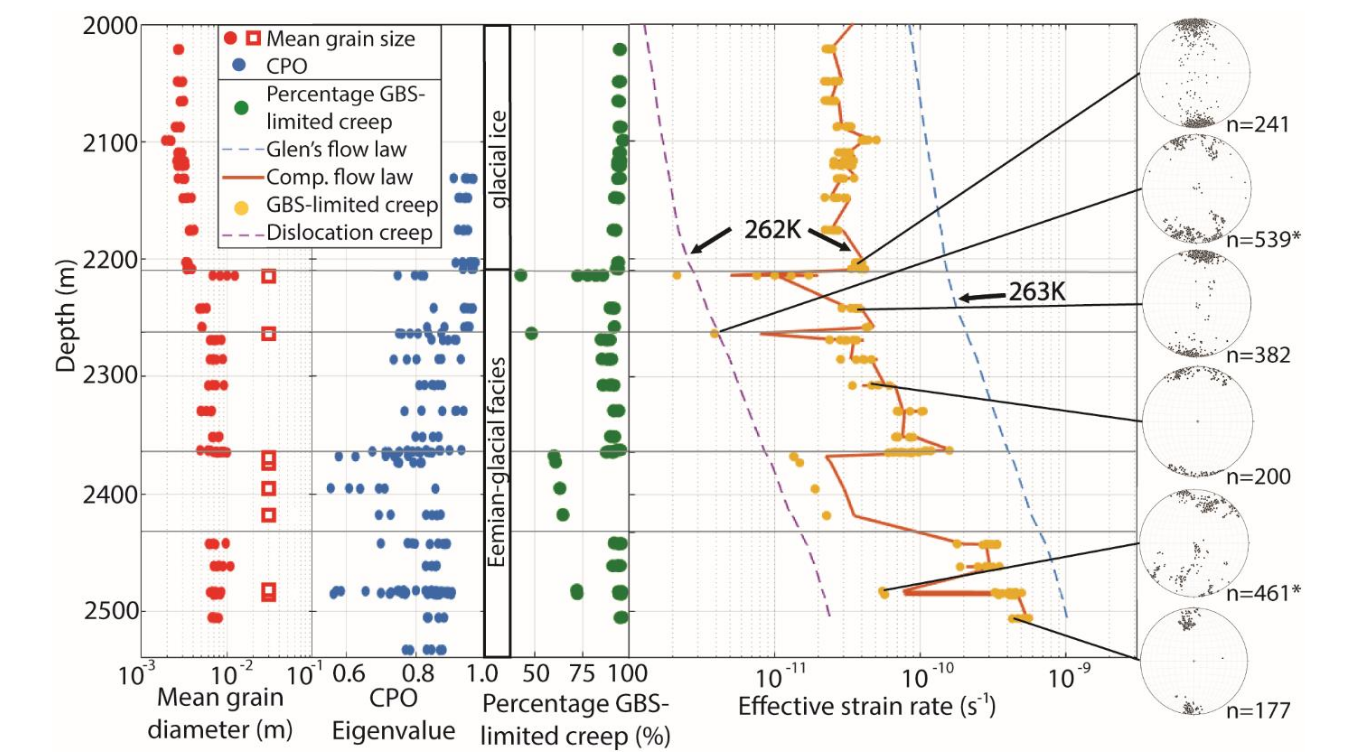
\includegraphics[width=11cm]{python_codes/fieldstone_59/images/kudd19}\\
{\captionfont Taken from Kuiper et al \cite{kudd19}.}
\end{center}

The conclusion from this exercise is that {\sl if} ice could be described by 
a linear viscous fluid flowing on an infinite incline, a viscosity of $\eta\simeq 10^{15}$Pa.s
would yield observations that match recorded velocities and strain rates. 


\paragraph{Nonlinear power-law viscosity}
However, the picture is way more complex, as it was observed very early on 
by Glen in 1955 \cite{glen55} and many others later (see Section~\ref{ss:glen}). 
It was then found that 
\[
\dot{\varepsilon} = A \tau^n,
\]
i.e. the ice behaves as a power-law fluid (see Section~\ref{ss:powerlaw}), with 
$n=3$ and $A\simeq 2.4\cdot 10^{-24}$ at 0\degree (REF?).

More recently Kuiper et al. \cite{kuwd19,kudd19} derived a composite flow law 
to model deformation in the NEEM deep ice core. 
They start from the flow law proposed by Goldsby \& Kohlstedt \cite{goko01}:
\[
\dot{\varepsilon}_T = \dot{\varepsilon}_{disl} + 
\left(\frac{1}{ \dot{\varepsilon}_{basal}} + \frac{1}{ \dot{\varepsilon}_{GBS}} \right)^{-1} 
+  \dot{\varepsilon}_{diff}
\]
where $\dot{\varepsilon}_T$  is the total strain rate, 
composed of strain rates for basal slip accommodated by non-basal slip or dislocation creep,
$\dot{\varepsilon}_{disl}$ , grain boundary sliding (GBS) accommodated by basal slip, 
$\dot{\varepsilon}_{basal}$ , and basal slip accommodated by GBS, 
$\dot{\varepsilon}_{GBS}$ , and diffusion creep, 
$\dot{\varepsilon}_{diff}$. Each of these creep mechanisms can be described by a 
power law relation of the form:
\[
\dot{\varepsilon} = A \tau^n d^{-p} \exp \left( -\frac{Q+pV}{RT} \right)
\]
where $A$ is a material parameter, $\tau$ is the differential stress (MPa), 
$n$ is the stress exponent, $d$ is the grain size diameter (m), 
$p$ is the grain size exponent, $Q$ is the activation energy for the creep 
mechanism at stake (J$\cdot$mol$^{-1}$ ), $p$ is the hydrostatic pressure (MPa), 
$V$ the activation volume (m$^3\cdot$mol$^{-1}$), 
$R$ is the gas constant (J$\cdot$K$^{-1}\cdot$mol$^{-1}$), and $T$ the absolute temperature (K). 
The effect of $pV$ is assumed to be very small \cite{dust01} 
and is ignored for the remainder of this work.

As explained in \cite{kuwd19} the composite flow law can actually be simplified to:
\[
\dot{\varepsilon}_T = \dot{\varepsilon}_{disl} + \dot{\varepsilon}_{GBS}
\]
The material parameters for these deformation mechanisms are available in \cite{kudd19}:
\begin{center}
\begin{tabular}{lcccc}
\hline
Creep regime & A & n & p & Q (J$\cdot$mol$^{-1}$) \\
\hline\hline
Glen's flow law ($T<263$K) &$3.61\cdot10^5$ MPa$^{-3.0}$ s$^{-1}$ &3.0 &0 &60\\
Glen's flow law ($T>263$K) &$1.73\cdot10^{21}$ MPa$^{-3.0}$ s$^{-1}$ &3.0 &0 &139\\
\hline
Dislocation creep ($T<262$K) & $5.0\cdot10^5$ MPa$^{-4.0}$ s$^{-1}$ &4.0 &0 &64\\
Dislocation creep ($T>262$K) &$6.96\cdot 10^{23}$ MPa$^{-4.0}$ s$^{-1}$ &4.0 &0 &155\\
\hline
GBS-limited creep ($T<262$K) & $1.1\cdot 10^2$ MPa$^{-1.8}$ m$^{1.4}$ $s^{-1}$ &1.8 &1.4 &70\\
GBS-limited creep ($T>262$K) & $8.5\cdot10^{37}$ MPa$^{-1.8}$ m$^{1.4}$ $s^{-1}$ &1.8 &1.4 &250\\
\hline
\end{tabular}
\end{center}

The associated effective viscosity is then given by 
\[
\eta = \frac{1}{2}  A^{-\frac{1}{n}} \dot{\varepsilon}^{\frac{1}{n}-1}  d^{\frac{p}{n}} \exp \left( \frac{Q+pV}{nRT} \right)
\]
Note that the $A$ parameter is given in MPa and not Pa so that when computing the 
associated effective viscosities these have to be multiplied by $10^6$.
Because the strain rates are added together we know that the two deformation mechanisms are in series and their
effective viscosity is then the harmonic average of both viscosities:
\[
\eta_{eff} = \left(\frac{1}{\eta_{disl}} + \frac{1}{\eta_{GBS}}  \right)^{-1}
\]

\paragraph{Numerical setup}

The geometry is a 2D cartesian domain of size $L_x \times L_y$. Instead of tilting it by an angle $\alpha$
I choose to instead 'tilt' the gravity vector so that it becomes 
$\vec{g}=(\rho g \sin_\alpha,-\rho g\cos\alpha)$.
The boundary conditions are as follows: no slip at the bottom, free surface at the top, 
free slip on the left (we assume that this corresponds to a ridge - zero horizontal velocity)
and we need to be careful about the right boundary which is where the ice exits the domain:
if we leave the boundary open ice will rush out, generate high strain rates and the nonlinear 
rheologies will respond by generating low viscosities which in turn will promote a fast 
exit. Instead we opt to prescribe the analytical solution of Eq.~(\ref{eq:ice1}) with $\eta=10^{15}$.
We neglect any kind of phase change and precipitation and only carry out a single time step.
The domain is discretised with nel=nelx$\times$nely $Q_2Q_1$ elements (see Section~\ref{ss:pairq2q1}).
We set $L_x=125$km and $L_y=2500$m, $\rho=917$kg$\cdot$m$^{-3}$, $\alpha=0.1$\degree.



\begin{center}
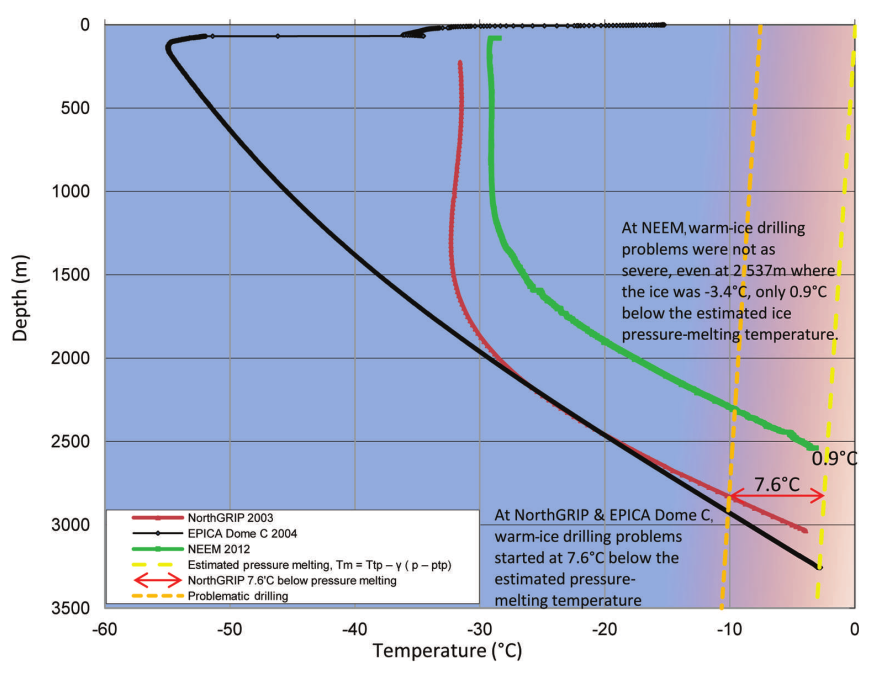
\includegraphics[width=6cm]{python_codes/fieldstone_59/images/shsh14}
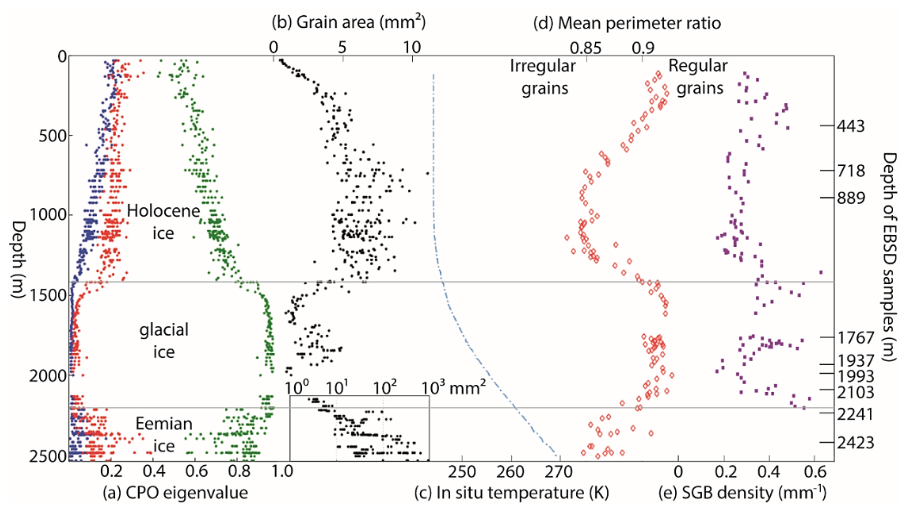
\includegraphics[width=8cm]{python_codes/fieldstone_59/images/kuiper19}\\
{\captionfont Left: Taken from Sheldon et al \cite{shsh14}; 
Right: Taken from Kuiper \cite{kuiper19}}
\end{center}

I have obtained the raw data (curtesy from E.N. Kuiper) and it is plotted hereunder:
\begin{center}
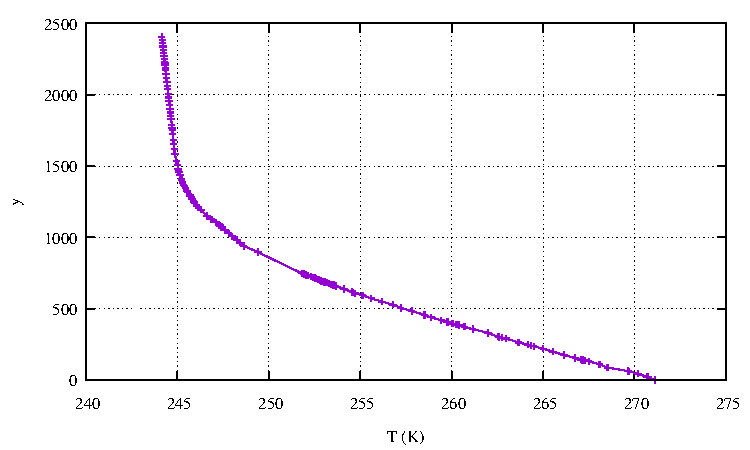
\includegraphics[width=7cm]{python_codes/fieldstone_59/data/temperature}
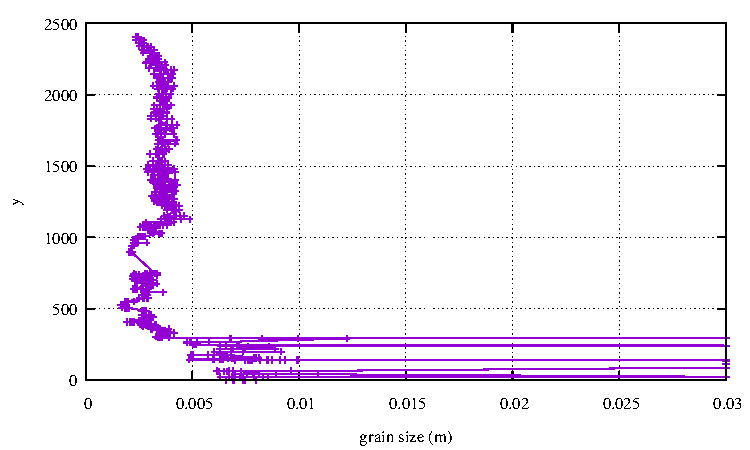
\includegraphics[width=7cm]{python_codes/fieldstone_59/data/grain_size}\\
{\captionfont }
\end{center}

In order to verify that the values reported in the table above are the ones 
used in \cite{kudd19} I have reproduced the figure 3 of that paper (code and gnuplot
script in {\sl ./data} folder):
\begin{center}
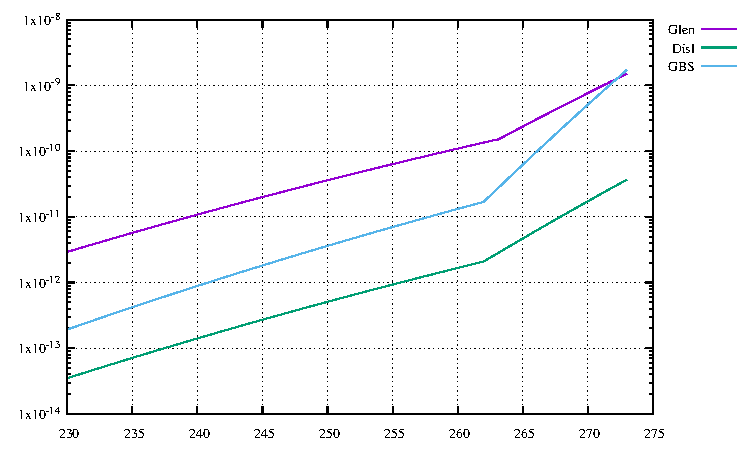
\includegraphics[width=8cm]{python_codes/fieldstone_59/data/strainrate}\\
{\captionfont Log strain rate versus temperature for Glen’s flow law and 
the two mechanisms (dislocation creep and GBS-limited creep) that form the end members 
of the modified composite flow law, using the flow law parameters from the table above. 
A stress of 0.07MPa and a mean grain diameter of 5mm were used to calculate the strain rate.}
\end{center}


In our models, the temperature profile is simplified 
as shown on the plots above. 
Concerning the grain size distribution the ice sheet has been divided in three 
layers and and an average grain size is used for each.

We have computed the effective viscosity for all four rheologies with the 
implemented temperature and grain size profiles for $\dot{\varepsilon}_e=10^{-10}\text{s}^{-1}$:

\begin{center}
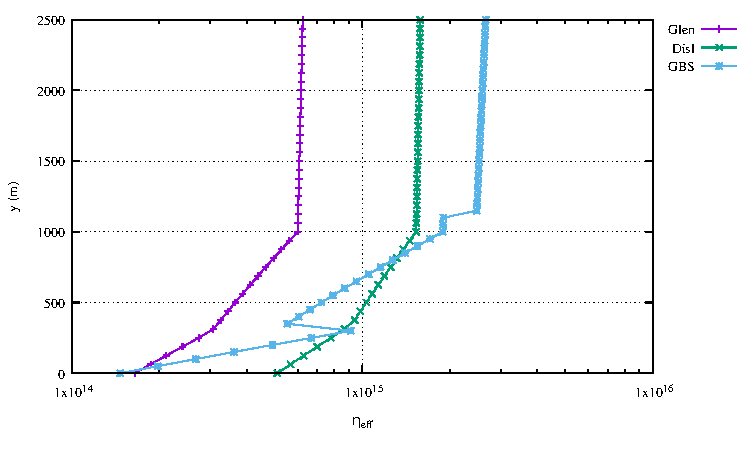
\includegraphics[width=7.5cm]{python_codes/fieldstone_59/results/profiles}
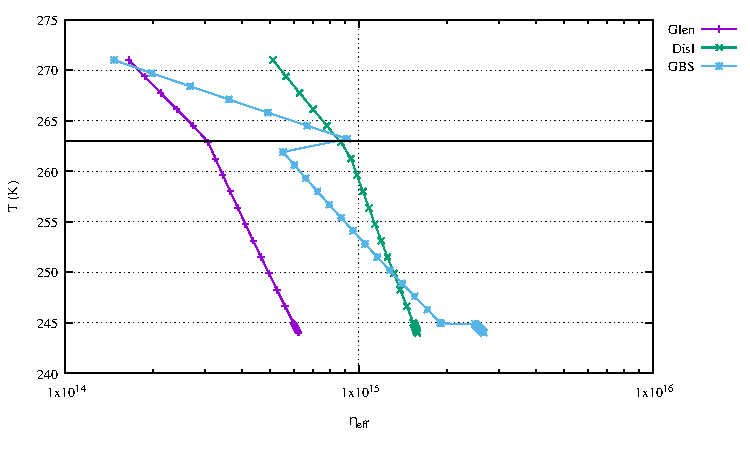
\includegraphics[width=7.5cm]{python_codes/fieldstone_59/results/profiles2}\\
\end{center}
Note that smaller strain rates shift the curves to the right (higher viscosities).



Because the rheologies are non linear we need to carry out nonlinear iterations (see Section~\ref{ss:picard}).
In what follows we run models for Glen's flow law (rheology=1), 
dislocation creep (rheology=2), GBS (rheology=3) and dislocation+GBS (rheology=4).
Note that in the case of rheology=4, the partitioning of the strain rates between both 
mechanisms is not done (YET) so that the results are not really consistent with the rest!

%\newpage
\begin{center}
Core 1 ($x=L_x/4$) \hspace{5cm}  Core 2 ($x=L_x/2$)  \\
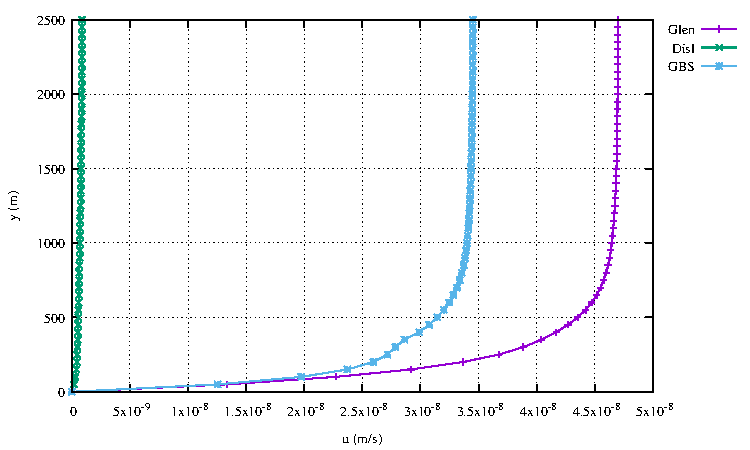
\includegraphics[width=7.cm]{python_codes/fieldstone_59/results/u_core1}
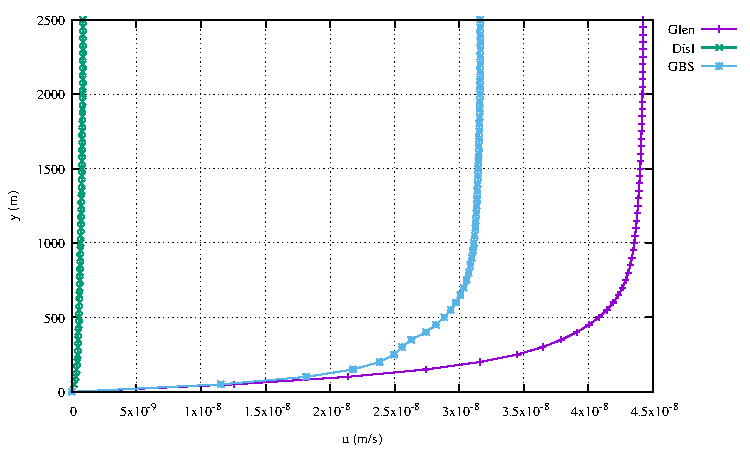
\includegraphics[width=7.cm]{python_codes/fieldstone_59/results/u_core2}\\
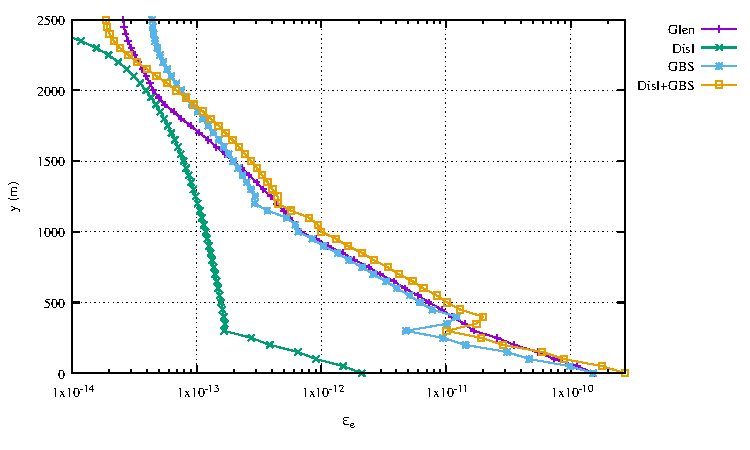
\includegraphics[width=7.cm]{python_codes/fieldstone_59/results/sr_core1}
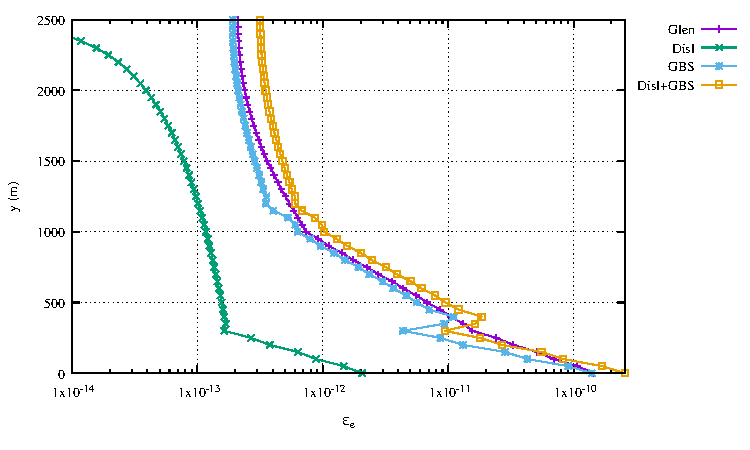
\includegraphics[width=7.cm]{python_codes/fieldstone_59/results/sr_core2}\\
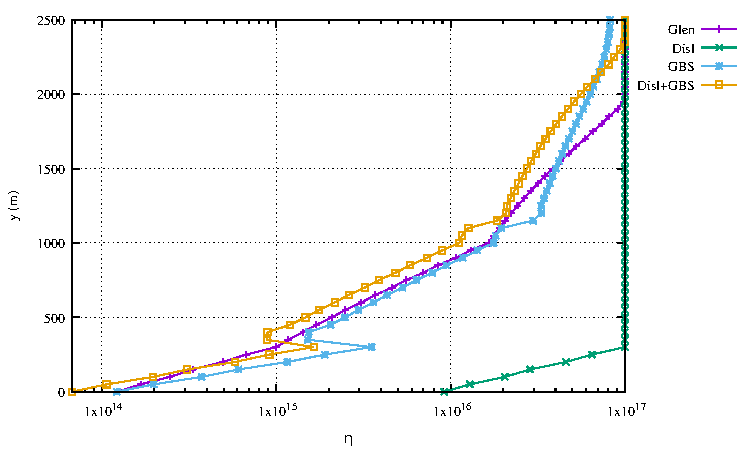
\includegraphics[width=7.cm]{python_codes/fieldstone_59/results/eta_core1}
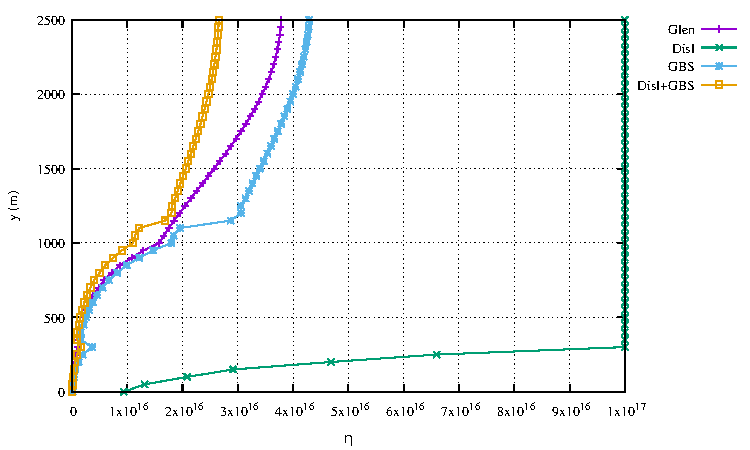
\includegraphics[width=7.cm]{python_codes/fieldstone_59/results/eta_core2}\\
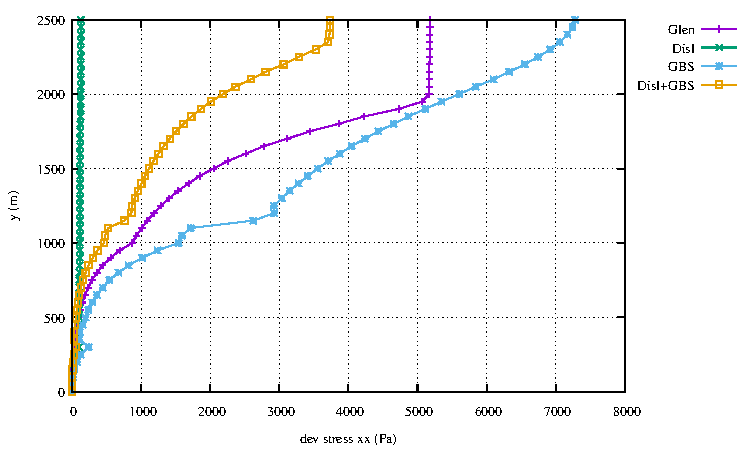
\includegraphics[width=7.cm]{python_codes/fieldstone_59/results/sigmaxx_core1}
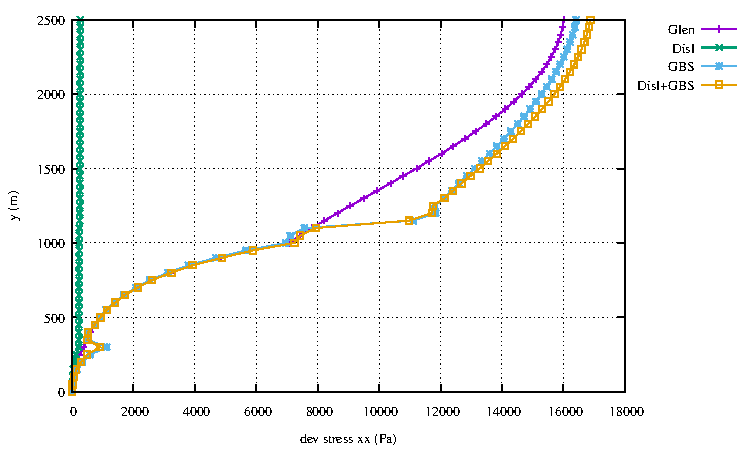
\includegraphics[width=7.cm]{python_codes/fieldstone_59/results/sigmaxx_core2}\\
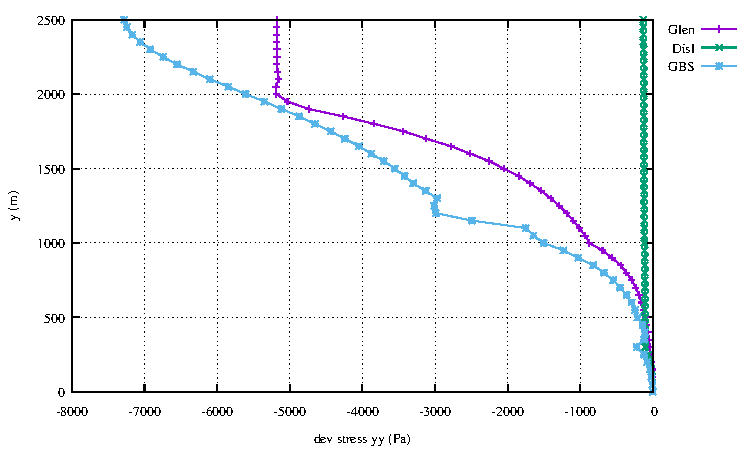
\includegraphics[width=7.cm]{python_codes/fieldstone_59/results/sigmayy_core1}
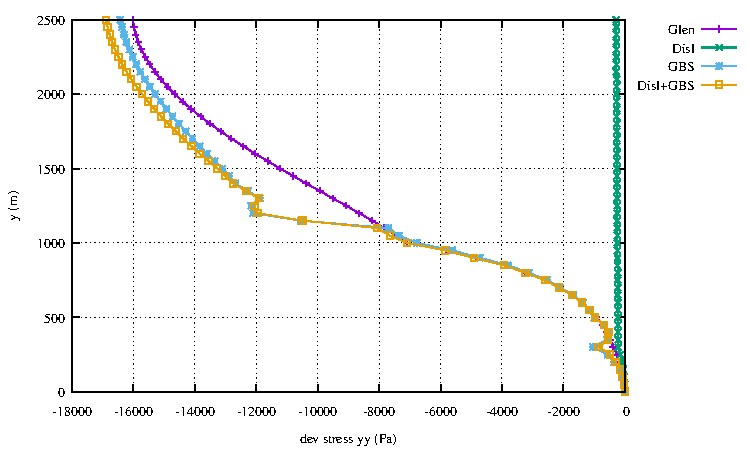
\includegraphics[width=7.cm]{python_codes/fieldstone_59/results/sigmayy_core2}\\
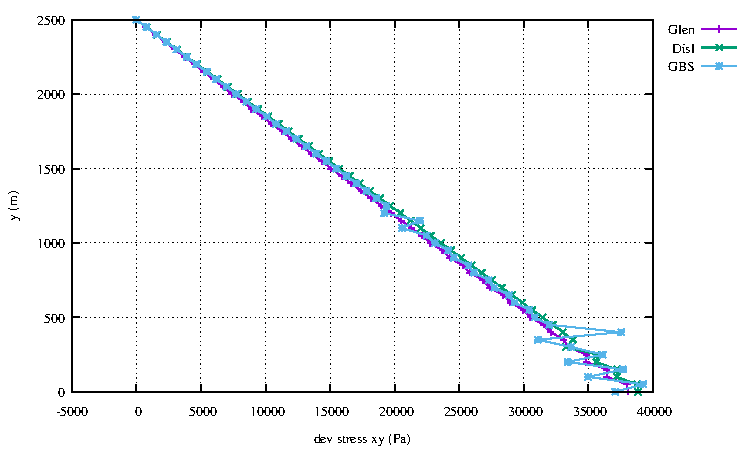
\includegraphics[width=7.cm]{python_codes/fieldstone_59/results/sigmaxy_core1}
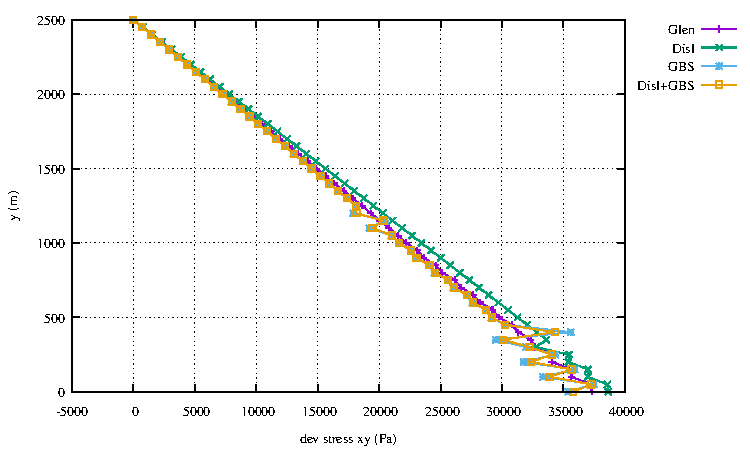
\includegraphics[width=7.cm]{python_codes/fieldstone_59/results/sigmaxy_core2}
\end{center}


\begin{center}
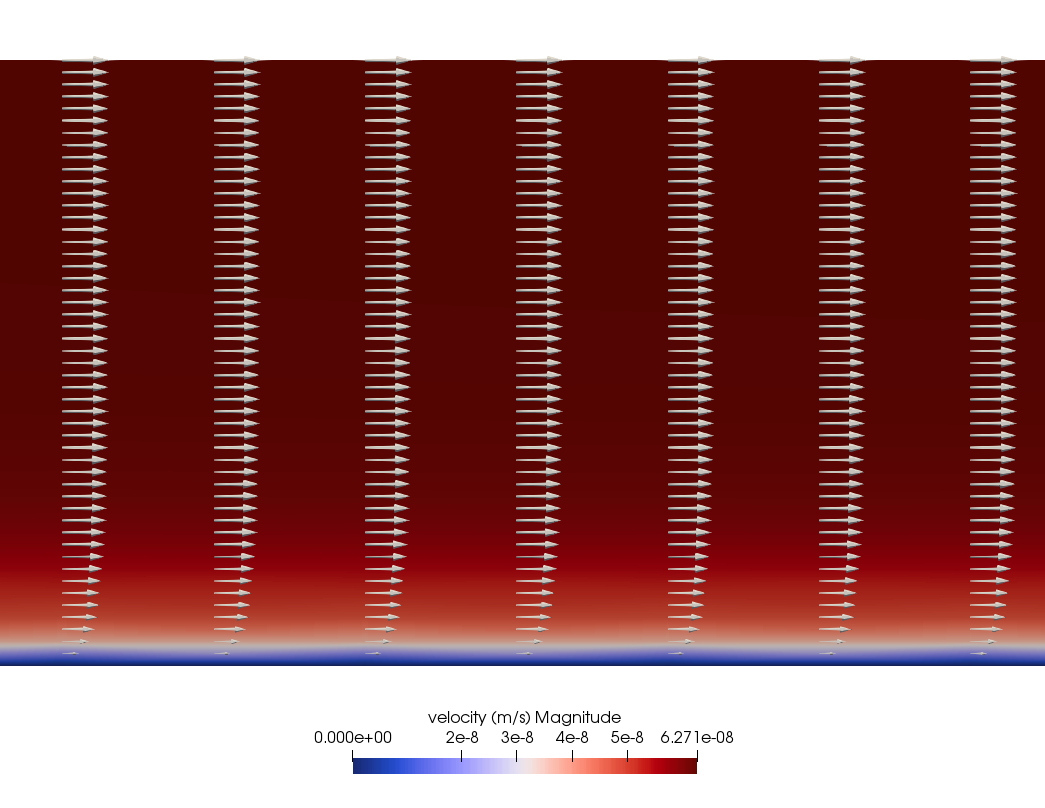
\includegraphics[width=6.cm]{python_codes/fieldstone_59/results/rh4/vel}
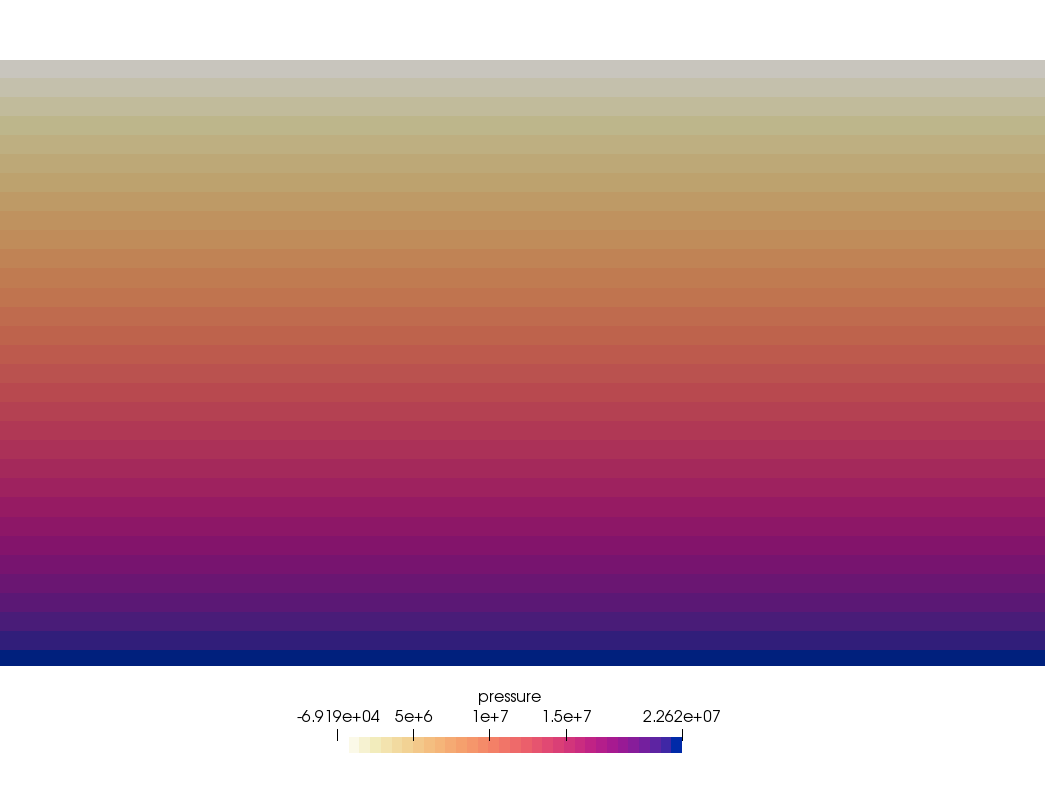
\includegraphics[width=6.cm]{python_codes/fieldstone_59/results/rh4/p}\\
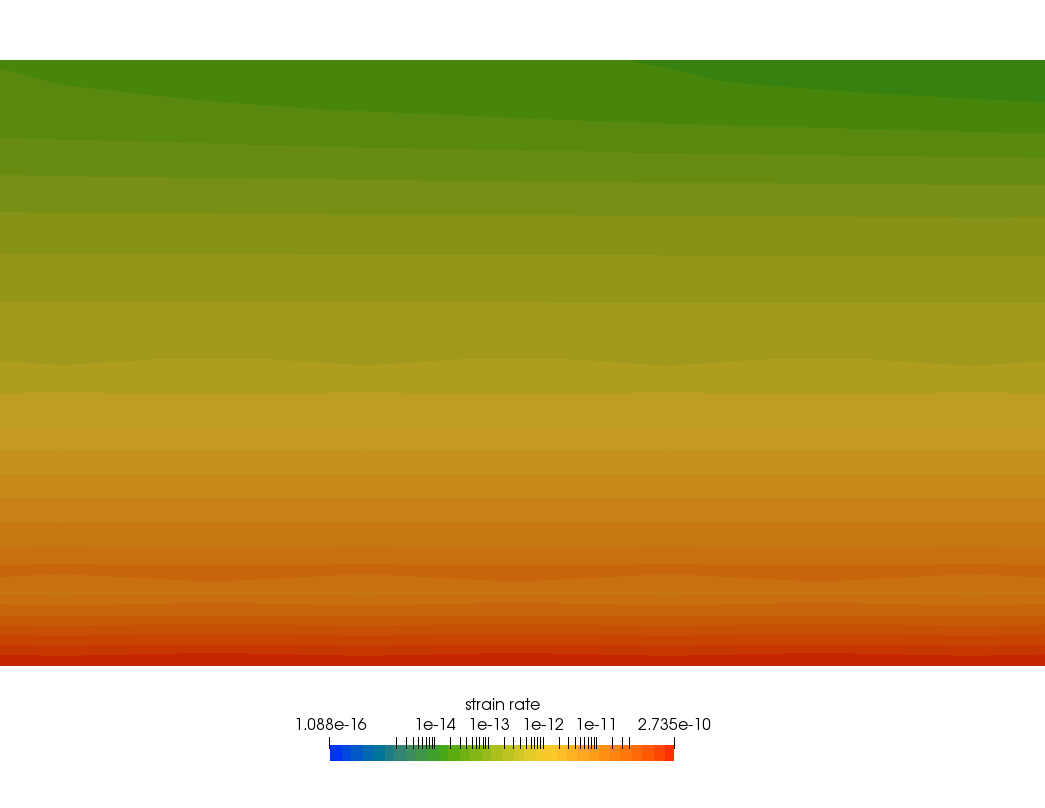
\includegraphics[width=6.cm]{python_codes/fieldstone_59/results/rh4/sr}
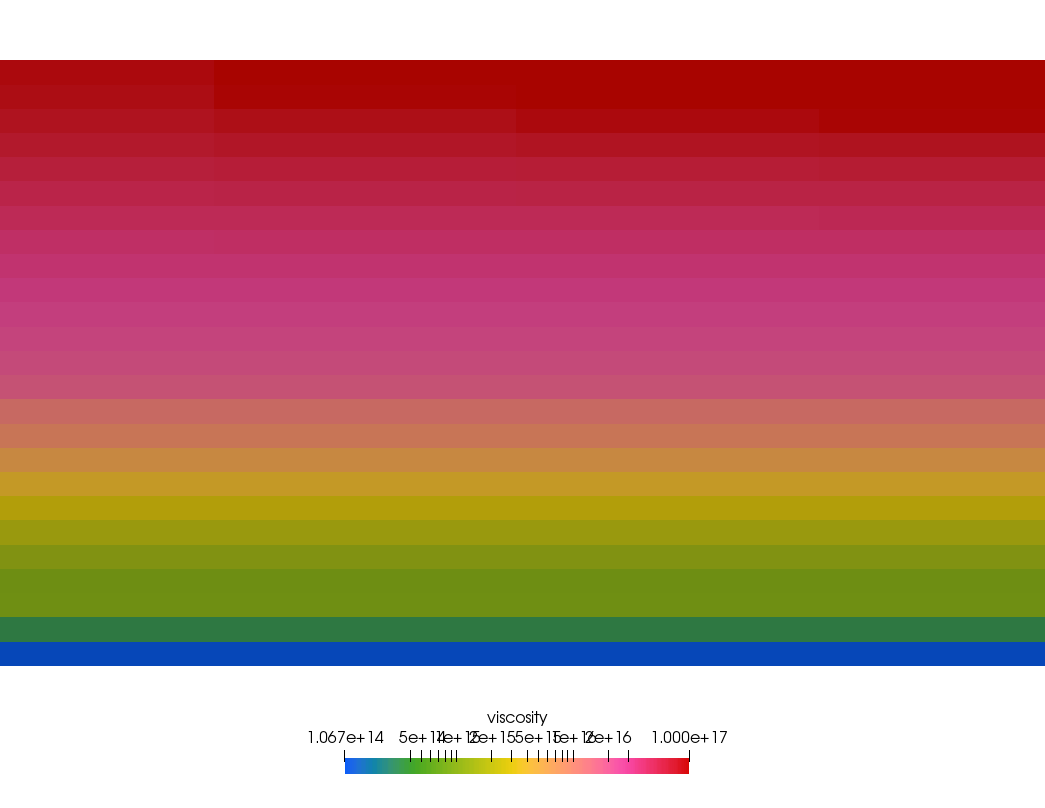
\includegraphics[width=6.cm]{python_codes/fieldstone_59/results/rh4/eta}\\
{\captionfont Velocity, pressure, strain rate and viscosity in the middle of the ice sheet
for rheology=4}
\end{center}



Check: ELMER/ice \url{http://elmerice.elmerfem.org/capabilities}

Improvements: better density profile? more realistic geometry ? 
partitioning of strain rates. Better temperature profile. 
Better grain size description. Influence of tilt angle? 



\vspace{1cm}

\Literature \cite{buja89}\cite{issg15}\cite{gors17}\cite{zhjg11}\cite{yash15}\cite{zwgg07}\cite{heah18}
\cite{lejx14}
